\pagebreak
\subsection{Results}
\label{ssec:results}
After all the development phases explained in section \ref{ssec:toolDev}, a tool with the required functionalities has been created (although it has some points to improve, as indicated in \ref{ssec:futureWork}), and \textbf{it is available in its Github repository\cite{ThisProjectGit}}.

%In the following sections, some examples of this tool execution in each system are shown, along with the trace they leave, which is one of the elements that need improvement. This part also has an example of how persistence can be applied in Active Directory.

%In the following section, an example of the tool execution on Linux is shown.
\subsubsection{External tools}

To test the external tool function, which is very interesting as it is capable of setting persistence to a backdoor tool, two different tools have been used:
\begin{itemize}
\item "Mistica"\cite{Mistica} for Linux, because it allows to establish communication using different protocols, even though this section is focused on the HTTPS protocol,
\item and "HTTP-revshell"\cite{HTTPRevshell} for Windows since it is written in PowerShell, simplifying its usage.
\end{itemize} 

To use them, the command to launch each one needs to be set in the parameter "HTTPScommand" of the "config.json" file.

\subsubsection{Use case}
These examples use a simple configuration file, and try to make persistent a simple script that writes an empty file in the user folder, which verifies that techniques worked. They also use their respective external tools to try to connect to a remote Linux server using an HTTPS connection.

%This example use a simple configuration file, provided before the execution, and try to make persistent a simple script that writes an empty file into the user folder, which verifies that all techniques worked.

\paragraph{Linux - Simple example}
For this example, the script shown in figure \ref{img:linpdaMaltest} has been provided as a payload.

\begin{figure}[!ht]
	%\hspace{-1.5cm}
	\centering
	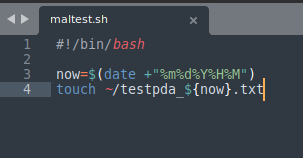
\includegraphics[width=8cm]{img/maltest}
	\caption{Dummy code in the file "maltest.sh".}
	\label{img:linpdaMaltest}
\end{figure}

\pagebreak
The configuration file, shown in figure \ref{img:linpdaConfigfile}, is set to only deploy "init" techniques on the user "user", which is the one used on this test. It also tries to establish a DNS connection, although it is not necessary for this technique.

\begin{figure}[!ht]
	%\hspace{-1.5cm}
	\centering
	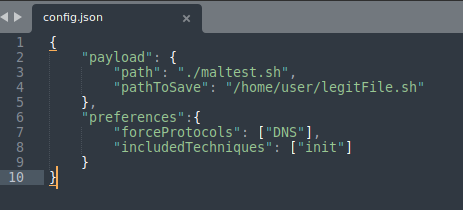
\includegraphics[width=12cm]{img/linPDA-configfile}
	\caption{Configuration file named "config.json".}
	\label{img:linpdaConfigfile}
\end{figure}

After all the files have been downloaded in the machine, the \texttt{home} and \texttt{Downloads} folders, and the \texttt{.bashrc} file have the content displayed in the figure \ref{img:linpdaBefore}.

\begin{figure}[!ht]
	%\hspace{-1.5cm}
	\centering
	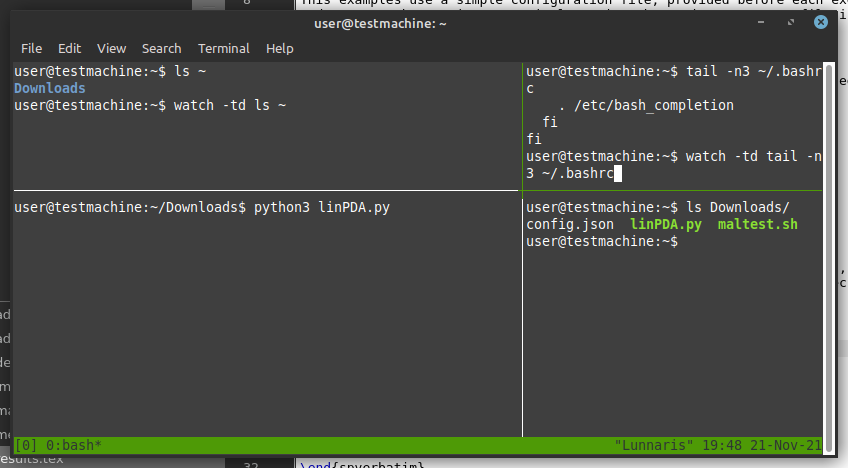
\includegraphics[width=14cm,trim={0.5cm 1cm 0.5cm 0.5cm},clip]{img/linPDA-before}
	\caption{Content of the folders and the \texttt{.bashrc} file before execution.}
	\label{img:linpdaBefore}
\end{figure}

In order to check the differences in the user folder and the \texttt{.bashrc} file after the execution of the script, the command \texttt{watch} is used to easily spot the changes, as it is a tool that executes other commands every few seconds.

\pagebreak
After the execution of the tool, a new file appears on "/home/user" and a new line is written in the "\texttt{.bashrc}" file, as can be seen in the following figure \ref{img:linpdaAfter}.

\begin{figure}[!ht]
	%\hspace{-1.5cm}
	\centering
	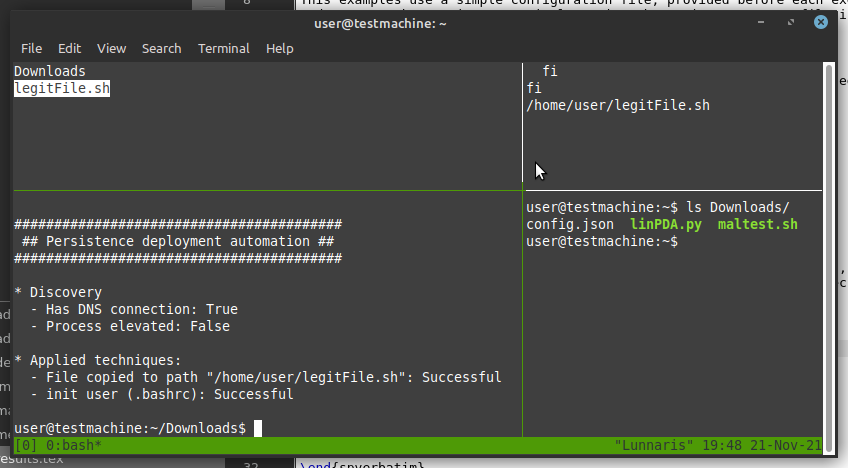
\includegraphics[width=14cm,trim={0.5cm 1cm 0.5cm 0.5cm},clip]{img/linPDA-after}
	\caption{Content of the folders and the \texttt{.bashrc} file after execution.}
	\label{img:linpdaAfter}
\end{figure}

In this case, only the \texttt{.bashrc} file is modified, as the user runs the script without privileges, as can be seen in the output of the script.

To end this example, now that the \texttt{.bashrc} file executes the copied script, a new file appears in the user home folder each time a new shell is opened, as can be seen in figure \ref{img:linpdaConsequences}.

\begin{figure}[!ht]
	%\hspace{-1.5cm}
	\centering
	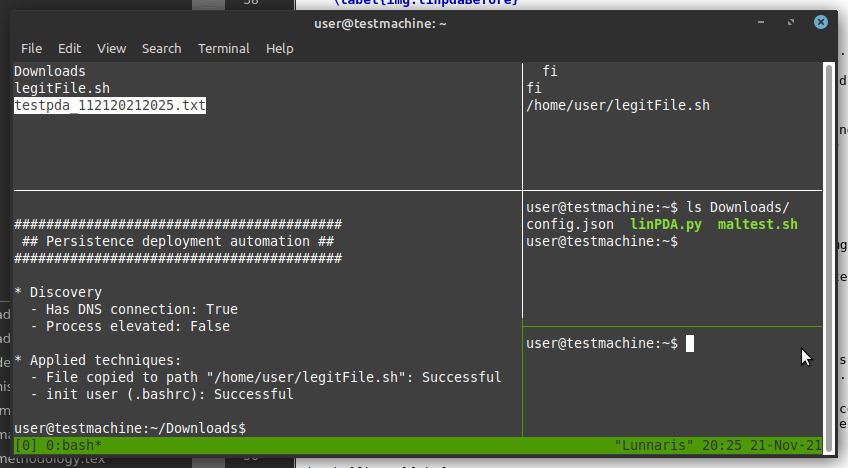
\includegraphics[width=14cm,trim={0.5cm 1cm 0.5cm 0.5cm},clip]{img/linPDA-consequences}
	\caption{New file in the home folder when a new bash terminal is opened.}
	\label{img:linpdaConsequences}
\end{figure}


\paragraph{Linux - HTTPS communication}
Using the same "maltest.sh" of the last example as a payload, shown in figure \ref{img:linpdaMaltest}, this time the persistence is deployed \underline{with elevated privileges} using the "crontab" technique, and an HTTPS tunnel is created with Mistica\cite{Mistica}.

The configuration file used is the one that is displayed in figure \ref{img:newlinPDAconfig}.

\begin{figure}[!ht]
	%\hspace{-1.5cm}
	\centering
	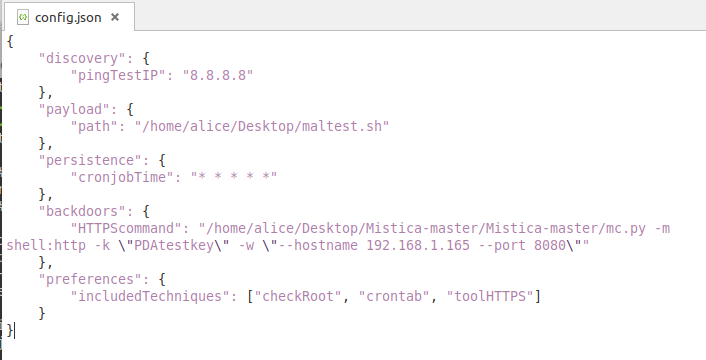
\includegraphics[width=14cm]{img/newlinPDA-config}
	\caption{Configuration file of the second example.}
	\label{img:newlinPDAconfig}
\end{figure}

As can be seen in the picture, Mistica needs the IP of the server to connect and its open port. This information relates also with figures \ref{img:newlinPDAsrvipconfig} and \ref{img:newlinPDAsrvstart}, where the server configuration can be observed.

\begin{figure}[!htb]
	%\hspace{-1.5cm}
	\centering
	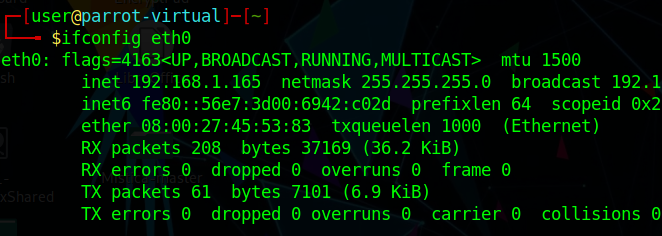
\includegraphics[width=14cm]{img/newlinPDA-ifconfigserver}
	\caption{IP address of the server.}
	\label{img:newlinPDAsrvipconfig}
\end{figure}

\begin{figure}[!htb]
	%\hspace{-1.5cm}
	\centering
	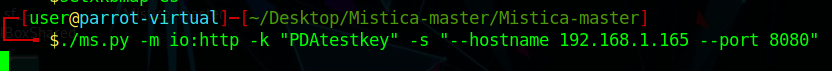
\includegraphics[width=14cm]{img/newlinPDA-servertstart}
	\caption{Command executed by the server.}
	\label{img:newlinPDAsrvstart}
\end{figure}

\pagebreak
Then, when everything is ready, the linux tool is executed, as can be seen in the following figures \ref{img:newlinPDAbeforewatch}, \ref{img:newlinPDAwatch} and \ref{img:newlinPDAexecuted}, where a windows watch the "/etc/crontab" file and the home directory for the user "alice".

\begin{figure}[!htb]
	%\hspace{-1.5cm}
	\centering
	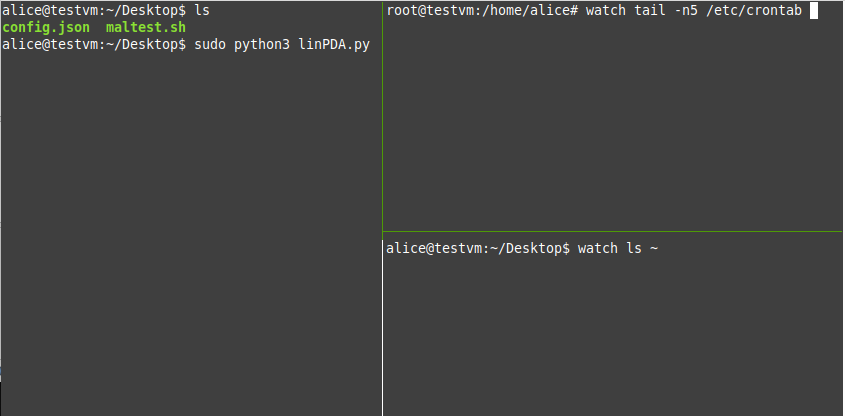
\includegraphics[width=14cm]{img/newlinPDA-watchready}
	\caption{Windows ready to watch changes.}
	\label{img:newlinPDAbeforewatch}
\end{figure}

\begin{figure}[!htb]
	%\hspace{-1.5cm}
	\centering
	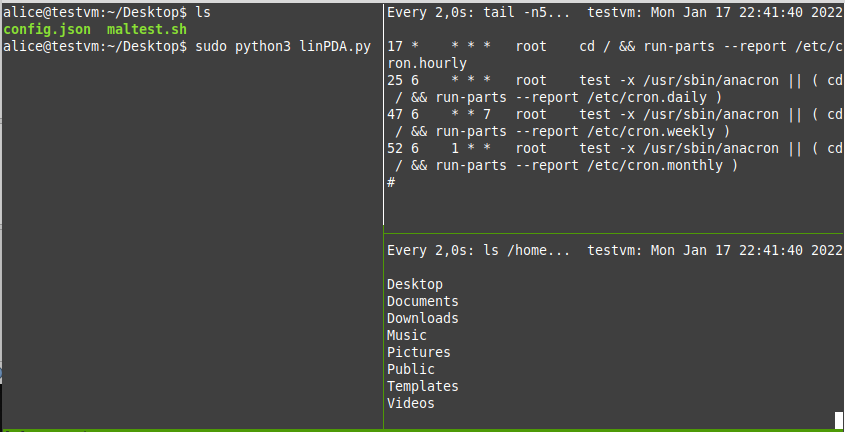
\includegraphics[width=14cm]{img/newlinPDA-watchexecuted}
	\caption{Windows watching for changes.}
	\label{img:newlinPDAwatch}
\end{figure}


\begin{figure}[!htb]
	%\hspace{-1.5cm}
	\centering
	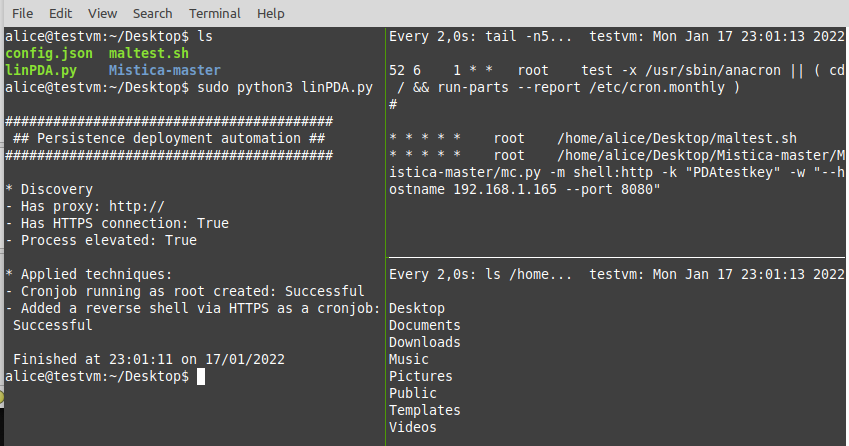
\includegraphics[width=14cm]{img/newlinPDA-executionOK}
	\caption{Changes appear and the command is executed correctly.}
	\label{img:newlinPDAexecuted}
\end{figure}

\pagebreak
Then, after a minute (as specified in the crontab), a new file can be spotted in the home directory, as it is shown in figure \ref{img:newlinPDAexeOKpost}, and also Wireshark, a tool that captures traffic, show some packets between the server and the host, as seen in the figure \ref{img:newlinPDAwireshark}.

\begin{figure}[!htb]
	%\hspace{-1.5cm}
	\centering
	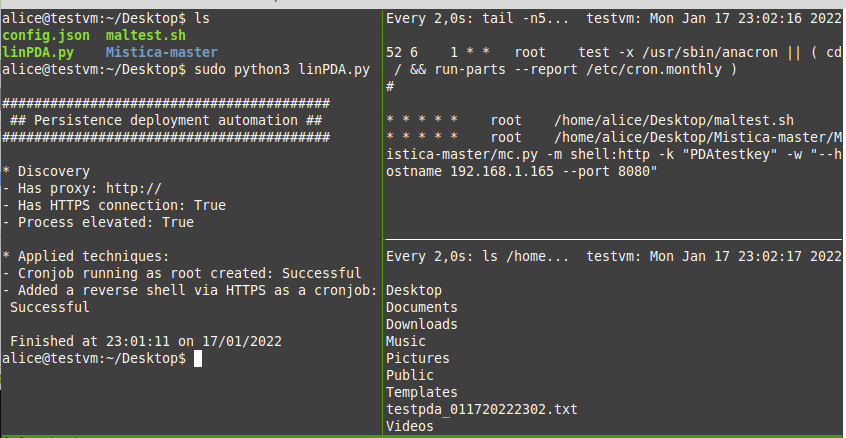
\includegraphics[width=14cm]{img/newlinPDA-executionOK-post}
	\caption{New file in the home folder.}
	\label{img:newlinPDAexeOKpost}
\end{figure}


\begin{figure}[!htb]
	%\hspace{-1.5cm}
	\centering
	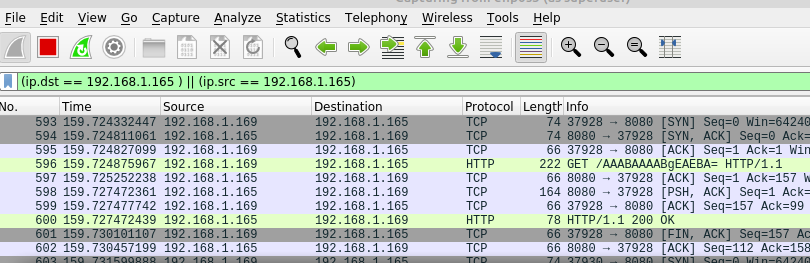
\includegraphics[width=14cm]{img/newlinPDA-wiresharkcapture}
	\caption{Packets captured with the Wireshark tool.}
	\label{img:newlinPDAwireshark}
\end{figure}

\pagebreak
Finally, as a reverse shell is being executed by Mistica, some commands can be executed on the host from the server, as can be seen in figure \ref{img:newlinPDAserverreverseshell}.

\begin{figure}[!htb]
	%\hspace{-1.5cm}
	\centering
	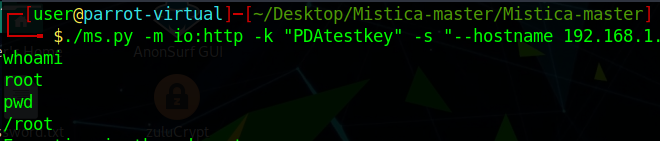
\includegraphics[width=14cm]{img/newlinPDA-serversuccess}
	\caption{Commands executed from the server into the host.}
	\label{img:newlinPDAserverreverseshell}
\end{figure}

\pagebreak

%\paragraph{Windows}
%[TODO]
%\subsubsection{Trails left after the deployment}

